\chapter{Cibles de fonctionnement}

\section{Les attentes client}

Nous avons été contactés par la société SPIE Sud-Est afin d'améliorer certains points dans le processus de gestion des contrats de maintenance. Il s'agit de proposer des solutions pour :

\begin{itemize}
    \item développement de procédures métier et de supports d'exploitation par les entités de maintenance et service
    \item standardisation des procédures métier et de supports d'exploitation pour les entités exerçant le même métier sur le même secteur d'activité client
    \item analyse des risques propres à chaque métier sur le même secteur d'activité client
    \item amélioration de la définition des limites des interfaces avec les autres processus
    \item mise en place d'un Info centre dur l'intranet
\end{itemize}

Les chapitres précédents --- analyse de l'existant et benchmarking -- permettent d'identifier quelques axes sur lesquels le système d'information de SPIE péche contre les bonnes pratiques et où des améliorations sont à prévoir.

    Nous allons donc citer dans ce document certains thèmes d'amélioration possibles à travers les axes suivant:

    \begin{enumerate}
        \item Réorganisation de la logique des processus existants~;
        \item Réorganisation des acteurs des processus métiers de SPIE pour suivre les ``best-practices'' dégagées~;
        \item Identification de nouvelles technologies à forte valeur ajoutée~;
    \end{enumerate}

\section{Réorganisation des processus}

\subsection{Processus Retour d'expérience}

Un premier probl\`eme que nous avions identifi\'e dans les processus actuels de SPIE-Sud-Est, est qu'il n'existe \`a l'heure actuel, aucun processus d\'edi\'e au retours que soit du client, ou des
differents intervenant sur le contrat. Pour cela, nous ajoutons donc trois nouveau processus au sous processus \textit{Solde de l'affaire et du contrat}~:

\begin{description}
    \item[Retour d'expérience client] afin que les clients puisses s'exprimer sur leurs \'experience avec SPIE~;
    \item[R\'eunion retour d'expérience interne] afin que les diff\'erents intervenant sur le contrat puisse communiquer les bon mais aussi movais points lors du deroulement du contrat e maniere
    interne~;
    \item[Bilan du contrat] afin de prendre en comptes l'ensemble des retours r\'ecolt\'e lors des \textit{Retour d'exp\'erience client} et de la \textit{R\'eunion retour d'expérience interne}.
\end{description}

\begin{figure}[h!]
	\centering
	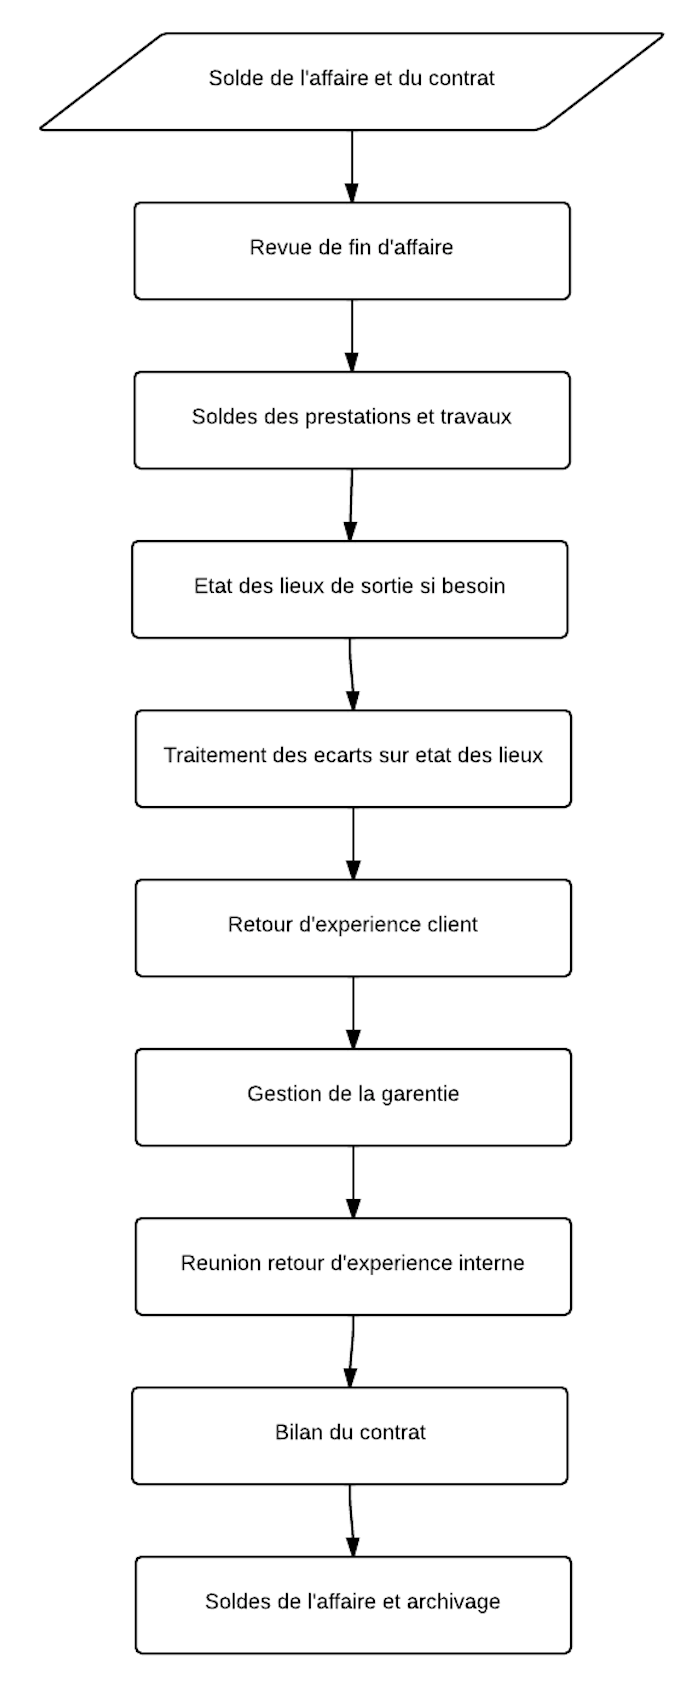
\includegraphics[width=0.45\linewidth]{images/processus_retour_experience.png}
	\caption{Sous processus Solde de l'affaire et du contrat}
	\label{fig:processusRetourExperience}
\end{figure}


\subsection{Revue des processus}

Le seconds soucis que nous avions identifi\'e dans les processus actuels de SPIE-Sud-Est, est qu'il n'y a aucun processus permettant une visibilit\'e sur l'ensemble des processus en cours ou aillant
\'et]'e clot. Alors nous prenons l'initiative de creer tout un processus indenpent et parrallele aux autres comportant deux processus~:

\begin{description}
    \item[Revues des processus sold\'es] uniquement d\'edi\'e au processus tout juste sold\'e depuis la derni\'ere revue, et notament globaliser les retour des processus \textit{Bilan du contrat}~;
    \item[Revues des processus en cours] quant \'a lui d\'edi\'e au processus en cours, afin de repartir les ressources materiel et humaines sur ces derniers.
\end{description}

\begin{figure}[h!]
	\centering
	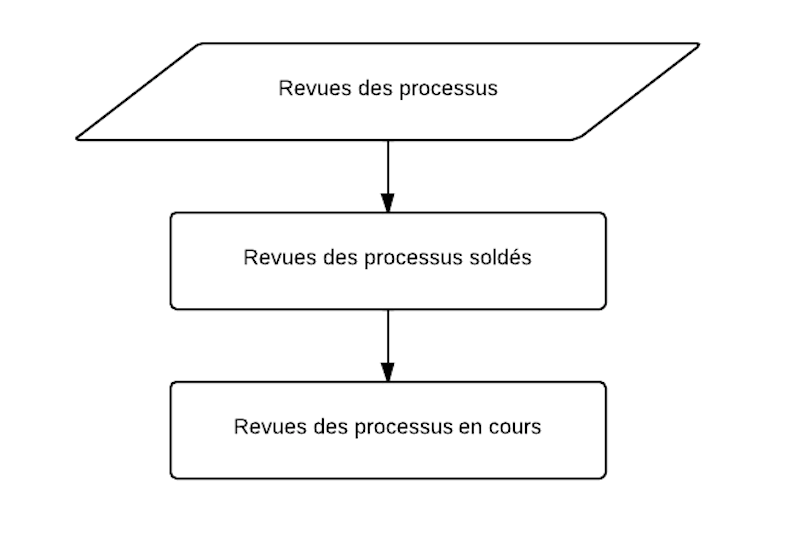
\includegraphics[width=0.45\linewidth]{images/processus_revues.png}
	\caption{Nouveau processus de revues}
	\label{fig:processusRevue}
\end{figure}

